% Options for packages loaded elsewhere
% Options for packages loaded elsewhere
\PassOptionsToPackage{unicode}{hyperref}
\PassOptionsToPackage{hyphens}{url}
\PassOptionsToPackage{dvipsnames,svgnames,x11names}{xcolor}
%
\documentclass[
  authoryear,
  3p]{elsarticle}
\usepackage{xcolor}
\usepackage{amsmath,amssymb}
\setcounter{secnumdepth}{5}
\usepackage{iftex}
\ifPDFTeX
  \usepackage[T1]{fontenc}
  \usepackage[utf8]{inputenc}
  \usepackage{textcomp} % provide euro and other symbols
\else % if luatex or xetex
  \usepackage{unicode-math} % this also loads fontspec
  \defaultfontfeatures{Scale=MatchLowercase}
  \defaultfontfeatures[\rmfamily]{Ligatures=TeX,Scale=1}
\fi
\usepackage{lmodern}
\ifPDFTeX\else
  % xetex/luatex font selection
\fi
% Use upquote if available, for straight quotes in verbatim environments
\IfFileExists{upquote.sty}{\usepackage{upquote}}{}
\IfFileExists{microtype.sty}{% use microtype if available
  \usepackage[]{microtype}
  \UseMicrotypeSet[protrusion]{basicmath} % disable protrusion for tt fonts
}{}
\makeatletter
\@ifundefined{KOMAClassName}{% if non-KOMA class
  \IfFileExists{parskip.sty}{%
    \usepackage{parskip}
  }{% else
    \setlength{\parindent}{0pt}
    \setlength{\parskip}{6pt plus 2pt minus 1pt}}
}{% if KOMA class
  \KOMAoptions{parskip=half}}
\makeatother
% Make \paragraph and \subparagraph free-standing
\makeatletter
\ifx\paragraph\undefined\else
  \let\oldparagraph\paragraph
  \renewcommand{\paragraph}{
    \@ifstar
      \xxxParagraphStar
      \xxxParagraphNoStar
  }
  \newcommand{\xxxParagraphStar}[1]{\oldparagraph*{#1}\mbox{}}
  \newcommand{\xxxParagraphNoStar}[1]{\oldparagraph{#1}\mbox{}}
\fi
\ifx\subparagraph\undefined\else
  \let\oldsubparagraph\subparagraph
  \renewcommand{\subparagraph}{
    \@ifstar
      \xxxSubParagraphStar
      \xxxSubParagraphNoStar
  }
  \newcommand{\xxxSubParagraphStar}[1]{\oldsubparagraph*{#1}\mbox{}}
  \newcommand{\xxxSubParagraphNoStar}[1]{\oldsubparagraph{#1}\mbox{}}
\fi
\makeatother


\usepackage{longtable,booktabs,array}
\usepackage{calc} % for calculating minipage widths
% Correct order of tables after \paragraph or \subparagraph
\usepackage{etoolbox}
\makeatletter
\patchcmd\longtable{\par}{\if@noskipsec\mbox{}\fi\par}{}{}
\makeatother
% Allow footnotes in longtable head/foot
\IfFileExists{footnotehyper.sty}{\usepackage{footnotehyper}}{\usepackage{footnote}}
\makesavenoteenv{longtable}
\usepackage{graphicx}
\makeatletter
\newsavebox\pandoc@box
\newcommand*\pandocbounded[1]{% scales image to fit in text height/width
  \sbox\pandoc@box{#1}%
  \Gscale@div\@tempa{\textheight}{\dimexpr\ht\pandoc@box+\dp\pandoc@box\relax}%
  \Gscale@div\@tempb{\linewidth}{\wd\pandoc@box}%
  \ifdim\@tempb\p@<\@tempa\p@\let\@tempa\@tempb\fi% select the smaller of both
  \ifdim\@tempa\p@<\p@\scalebox{\@tempa}{\usebox\pandoc@box}%
  \else\usebox{\pandoc@box}%
  \fi%
}
% Set default figure placement to htbp
\def\fps@figure{htbp}
\makeatother





\setlength{\emergencystretch}{3em} % prevent overfull lines

\providecommand{\tightlist}{%
  \setlength{\itemsep}{0pt}\setlength{\parskip}{0pt}}



 
\usepackage[]{natbib}
\bibliographystyle{elsarticle-harv}


\usepackage{gb4e}
\noautomath
% \usepackage[inline]{glossaries}
\usepackage{leipzig}
% \makeglossaries
\usepackage{typgloss}
\usepackage{setspace}
\usepackage{lineno}
\linenumbers
\usepackage{booktabs}
\usepackage{longtable}
\usepackage{array}
\usepackage{multirow}
\usepackage{wrapfig}
\usepackage{float}
\usepackage{colortbl}
\usepackage{pdflscape}
\usepackage{tabu}
\usepackage{threeparttable}
\usepackage{threeparttablex}
\usepackage[normalem]{ulem}
\usepackage{makecell}
\usepackage{xcolor}
\makeatletter
\@ifpackageloaded{caption}{}{\usepackage{caption}}
\AtBeginDocument{%
\ifdefined\contentsname
  \renewcommand*\contentsname{Table of contents}
\else
  \newcommand\contentsname{Table of contents}
\fi
\ifdefined\listfigurename
  \renewcommand*\listfigurename{List of Figures}
\else
  \newcommand\listfigurename{List of Figures}
\fi
\ifdefined\listtablename
  \renewcommand*\listtablename{List of Tables}
\else
  \newcommand\listtablename{List of Tables}
\fi
\ifdefined\figurename
  \renewcommand*\figurename{Figure}
\else
  \newcommand\figurename{Figure}
\fi
\ifdefined\tablename
  \renewcommand*\tablename{Table}
\else
  \newcommand\tablename{Table}
\fi
}
\@ifpackageloaded{float}{}{\usepackage{float}}
\floatstyle{ruled}
\@ifundefined{c@chapter}{\newfloat{codelisting}{h}{lop}}{\newfloat{codelisting}{h}{lop}[chapter]}
\floatname{codelisting}{Listing}
\newcommand*\listoflistings{\listof{codelisting}{List of Listings}}
\makeatother
\makeatletter
\makeatother
\makeatletter
\@ifpackageloaded{caption}{}{\usepackage{caption}}
\@ifpackageloaded{subcaption}{}{\usepackage{subcaption}}
\makeatother
\journal{Cognition}
\usepackage{bookmark}
\IfFileExists{xurl.sty}{\usepackage{xurl}}{} % add URL line breaks if available
\urlstyle{same}
\hypersetup{
  pdftitle={(In)sensitivity to surface-level heuristics: A case from Turkish verbal attractors},
  pdfauthor={Utku Turk},
  pdfkeywords={form-sensitivity, memory, agreement attraction},
  colorlinks=true,
  linkcolor={blue},
  filecolor={Maroon},
  citecolor={Blue},
  urlcolor={Blue},
  pdfcreator={LaTeX via pandoc}}


\setlength{\parindent}{6pt}
\begin{document}

\begin{frontmatter}
\title{(In)sensitivity to surface-level heuristics: A case from Turkish
verbal attractors}
\author[1]{Utku Turk%
\corref{cor1}%
}
 \ead{utkuturk@umd.edu} 

\affiliation[1]{organization={University of Maryland, College
Park, Linguistics},addressline={Marie Mount Hall},city={College
Park},postcode={20742},postcodesep={}}

\cortext[cor1]{Corresponding author}

        
\begin{abstract}
We ask whether surface-form overlap alone can elicit agreement
attraction or whether attraction requires morphosyntactic features that
(possibly) license controllerhood. Turkish provides a test case because
the plural morpheme \emph{-lAr} appears on both nouns and verbs, but
only nominal \emph{-lAr} can control verbal agreement. In two speeded
acceptability experiments with Turkish, we show that the association
with being a possible controller is needed for surface-level heuristics
to kick in. In Experiment 1 (N = 80) we used reduced relative clauses
whose verb bore \emph{-lAr} as potential verbal attractors and compared
ungrammatical sentences with plural vs.~singular verbal attractors.
Ungrammatical sentences with a plural-marked verbal attractor were not
judged more acceptable than those with a singular verbal attractor. In
Experiment 2 (N = 95) we replicated the verbal manipulation and added
genitive-marked nominal attractors; nominal plural attractors produced
robust attraction, but verbal plural attractors did not. The
within-experiment distribution influenced baseline acceptability, yet it
did not create attraction for verbal attractors. The results indicate
that surface similarity alone is insufficient. Attraction depends on
abstract feature overlap with elements that can serve as agreement
controllers, not on the presence of a homophonous plural morpheme on a
non-controller.
\end{abstract}





\begin{keyword}
    form-sensitivity \sep memory \sep 
    agreement attraction
\end{keyword}
\end{frontmatter}
    

\section{Introduction}\label{introduction}

Sentence processing is shaped not only by grammatical constraints but
also by plausibility, frequency, task-specific factors, and phonological
processes. Recent work shows that such influences can substantially
modulate reading and judgment behavior
\citep{LauraMalsbug24, ArehalliWittenberg2021, HammerlyEtAl2019, LogacevVasishth2016}.
Form-based overlap between elements in a sentence can also influence how
sentences are processed. A substantial body of work has shown that the
parser and the production system are sensitive not only to syntactic or
semantic relations but also to the surface form of words. These effects
have been taken to suggest that, under certain circumstances, speakers
and comprehenders rely on shallow or heuristic cues to complete
dependencies. \citet{AchesonMacDonald2011}, for example, found that
participants showed slower reading times when the subjects of the two
embedded clauses share phonological similarity
(\emph{baker}-\emph{banker} in \ref{baker}
vs.~\emph{runner}-\emph{banker} in \ref{runner}). Moreover, participants
were less accurate in answering comprehension questions with
phonological overlap present. Related work in short-term memory and word
recognition shows similar effects---items that overlap phonologically or
morphologically are more confusable and more easily retrieved
\citep{CopelandRadvansky2001, RastleDavis2008}.

\begin{exe}
\ex \label{baker} The baker that the banker sought bought the house.
\ex \label{runner} The baker that the banker sought bought the house..
\end{exe}

\begin{itemize}
\tightlist
\item
  Here I should put Kush actually debunked this.
\end{itemize}

One domain in which these influences are observed is the research on
agreement attraction as in (\ref{og}), a phenomenon in which a verb
erroneously agrees with a nearby noun rather than its grammatical
subject, producing so-called grammaticality illusions
\citep{BockMiller:1991, PearlmutterGarnseyBock:1999}. This effect have
been robustly attested in many languages with various methodologies
{[}to name a few{]}. \citet{BockEberhard1993} tested whether attractors
that only sound plural, pseudoplurals such as \emph{course}
\ref{pseudo}, increase agreement errors compared to true plural nouns
(\ref{true-pl}). They reasoned that if participants rely on phonological
cues rather than abstract features, words ending with plural-like sounds
(/s/ or /z/) should behave like true plurals. Participants completed
sentence preambles such as (\ref{ex:bockeberhard93}), where the head
noun (\emph{player}) was singular but the attractor varied in form. They
found that pseudoplural attractors did not increase plural agreement
rates.

\begin{exe}
\ex[*]{\label{og} The player on the courts are tired from a long-game.}
\ex \label{ex:bockeberhard93}
\begin{xlist}
    \ex \label{pseudo} {Pseudoplural Attractor} \\ The {player} on the {course} \ldots{}
    \ex \label{true-sg} {Singular Attractor} \\ The {player} on the {court} \ldots{}
    \ex \label{true-pl} {Plural Attractor} \\ The {player} on the {courts} \ldots{}
\end{xlist}
\end{exe}

Even though modulation from a pure phonological similarity was not
found, several experiments have manipulated morphological case
similarity between controllers and attractors, reasoning that syncretism
or surface ambiguity could enhance competition during retrieval or
interfere in production {[}PAPERS{]}. For example,
\citet{HartsuikerEtAl2003} used the overlap between accusative and
nominative forms of feminine determiners in German and compared these
ambiguous forms to distinctively marked dative forms. Participants
produced more agreement errors when the preambles contained two noun
phrases whose determiners were not distinctively marked, as in
(\ref{ger-amb}), compared to cases where the attractor could be
distinguished by form alone, as in (\ref{ger-dist}). Crucially, this
additive effect was limited to feminine nouns, the only gender showing
nominative--accusative syncretism in plural forms while other nouns
showed the base effect of plural.

\begin{exe}
\ex \label{ger}
\begin{xlist}
\ex \label{ger-amb}
\gll Die Stellungnahme gegen die Demonstration-en\\
the.F.NOM.SG position against the.F.ACC.PL demonstration-PL\\
\glt `The position against the demonstrations'
\ex \label{ger-dist}
\gll Die Stellungnahme zu den Demonstration-en\\
the.F.NOM.SG position on the.F.DAT.PL demonstration-PL\\
\glt `The position on the demonstrations'
\end{xlist}
\end{exe}

Similar effects of surface similarity are also found in comprehension
studies. \citet{Slioussar2018}, for example, showed that phonological
overlap affects the reading pattern and accuracy of participants in
Russian agreement. A group of accusative marked nouns in Russian
surfaces ambiguously with their nominative counterparts when they are
plural (\ref{RusAccSg}-\ref{RusAccPl}). Meanwhile, it is possible to
assign a different case to the attractors using a different preposition
as in (\ref{RusGenSg}-\ref{RusGenPl}). Crucially, in her experiment the
genitive marked plural nouns were not ambiguous with their nominative
counterparts. \citet{Slioussar2018} showed that participants not only
exhibited faster reading times at the verb in (\ref{RusAccPl}) compared
to (\ref{RusAccSg}), but also judged sentences with a plural attractor
as grammatical more often. These effects of plural attractor were only
present in cases with ambiguous case marking.

\begin{exe}
\ex
\begin{xlist}
\ex \label{RusAccSg}
\gll ssylka na sajt byli dany.\\
link[NOM.SG] to {website[ACC.SG($\neq$NOM.PL)]} were given\\
\ex \label{RusAccPl}
\gll ssylka na sayty byli dany.\\
link[NOM.SG] to {website[ACC.PL($=$NOM.PL)]} were given\\
\glt `The link to the website(s) were given.'
\ex \label{RusGenSg}
\gll material dlja kry\c{s}i byli brakovannymi.\\
material[NOM.SG] for {roof[GEN.SG($=$NOM.PL)]} were defective\\
\ex \label{RusGenPl}
\gll material dlja kry\c{s} byli brakovannymi.\\
material[NOM.SG] for {roof[GEN.PL($\neq$NOM.PL)]} were defective\\
\glt `The material for the roof(s) were defective.'
\end{xlist}
\end{exe}

However, a more intriguing aspect of the study by \citet{Slioussar2018}
is her results with respective to attractors marked with genitive
singular. Another interesting characterics of Russian is such that a
subset of \emph{singular} genitive nouns share the same form with their
plural nominal counterpart. In addition to plural nouns not increasing
grammatical judgments to ungrammatical sentences and not creating a
reading advantage, the verbs of singular attractors were read faster and
resulted in more `yes' responses to grammaticality judgments. In this
aspect, the findings of \citet{Slioussar2018} differs from previous
syncretism findings and targets the initial question raised by
\citet{BockEberhard1993}: whether the pure phonological similarity,
without any contribution from an abstract plural feature, can drive the
agreement attraction effects.

\citet{Slioussar2018} assumed cue-based retrieval model in which
attraction effects originates from erroneous retrievals of an agreement
controller. Under this approach, phrases are encoded in a
content-addressable memory as bundles of features called \emph{chunks}
which include information like, number, gender, morphophonological case,
and syntactic information \citep{SmithVasishth2020, LV05}. Participants
predict the number of the verb based on the noun phrases they process
while reading the previous noun phrases. In grammatical sentences with
singular verb agreement, the number prediction and the verb number
match, which causes no processing difficulty. In contrast, when
participants fail to find the predicted number morphology on the verb, a
memory-retrieval process is initiated. This process activates the search
for a chunk matching relevant cues for agreement controller.
\citet{Slioussar2018} argued that the search for a controller can be
mediated through possible forms of nouns with relevant features like,
\textsc{nom} case, \textsc{pl} number, as well as structural cues.

In ungrammatical sentences like (\ref{RusAccPl}), while neither of the
available noun phrases fully matches this specification in ungrammatical
agreement attraction sentences, each of the NPs headed by \emph{link}
and \emph{websites} matches a subset of cues. Importantly, in
(\ref{RusGenSg}) as well, a partial match is also possible. Even though
the NP headed by \emph{roof} is not plural, due to phonological overlap,
\citet{Slioussar2018} argues, a subset of features relevant for
agreement, i.e.~+NOM and +PL, is erroneously activated. While this
partial match scenarios mostly results in participants finding the
sentence ungrammatical, they may occasionally retrieve the attractors,
\emph{websites} or \emph{roof}, as controllers on some trials.

An alternative account that does not depend on activation of relevant
features by phonology would depend on encoding of distributional facts
as statistical heuristics. In such an account, instead of relying on
activation of features through a phonological route, participants would
probabilistically associate certain strings, such as genitive marked NP
or overt D head, with being an agreement controller. Indeed, similar
explanations for syncretism or subject-likeness phenomenon has been
reported. For example, \citet{LagoEtAl2019} argued that participants can
retrieve a noun as the controller if the noun is marked with a case
marking that may sometimes control agreement in a language even if that
is not the case for the specific sentence. They used Turkish genitive
case, which can control the agreement in embedded sentences but not in
matrix sentences. They took the presence of attraction effects in
Turkish as an indication that Turkish speakers utilize overt
genitive-case's association with subjecthood. In a sense, phonological,
not functional, syncretism between the marking on the nominal modifier
and the embedded subject resulted in attraction. A similar account from
Dillon and colleagues was pushed for sensitivity for looking like a
controller in languages like Romanian and Hindi
\citep{BhatiaDillon2022, BleotuDillon2024}. For instance,
\citet{BleotuDillon2024} manipulated whether the attractor surfaces with
a determiner or in its bare form. Importantly, they note that only nouns
with determiners can control agreement in Romanian. They found that
Romanian attractors only induced attraction effects when both attractor
and the head surfaced with a determiner. They took these results to
suggest that participants associated presence of a determiner or related
feature with the agreement controller, and attraction only surfaces when
subject heads and the attractor look alike. Similarly,
\citet{SchlueterEtAl2018} argue that and can cause agreement attraction
effects in English even when it does not create a plurality because it
is associated with the plural feature statistically. Such explanations
are based on the assumption that the match between a cue and a chunk
does not have to be categorical, but it can be influenced by surface
level statistical association \citep{EngelmannEtAl2019}.

A similar account can also be proposed for Russian findings. Genitive
marked nouns can be subjects in negative inversion constructions in
Russians. However, when they are subjects, they cannot control the
agreement. In other cases, they can be the controller of number or
gender marking on adjectival relative clauses. Given this possibility of
an alternative account, the contention of initial findings of
\citet{BockEberhard1993}, and the theoretical importance of the
empirical generalization, we test whether pure phonological overlap can
derive agreement attraction effects in two high-powered speeded
acceptability judgment experiments. To this end we use Turkish, a
language where verbal and nominal plural marking share the same surface
form, the suffix --lAr. We use reduced relative clause (RRC) structures,
in which the verb with the plural marking alone can appear as the
attractor (\ref{rrc-intro}). Importantly, Turkish --lAr syncretism here
is not feature-ambiguous (as in cases of syncretism); it is a form-only
overlap that does not share possible argument status with the subject.
Even when the RRC can surface without its head as the subject, they
cannot control the agreement (\ref{rrc-subject}).

\begin{exe}
\ex \label{rrc-intro}
\gll Gör-dük-ler-i çocuk koş-tu-(*lar).\\
go-NMLZ-PL-POSS kid[NOM] run-PST-(*PL)\\
\glt `The kid that (they) saw ran.'
\ex \label{rrc-subject}
\gll Gör-dük-ler-i koş-tu-(*lar).\\
go-NMLZ-PL-POSS run-PST-(*PL)\\
\glt `(The kid) that (they) saw ran.'
\end{exe}

In Experiment 1, we tested the form hypothesis directly by comparing
ungrammatical sentences with verbal-plural vs.~verbal-singular
attractors. Experiment 2 replicated this design but included additional
nominal-attractor items from a previous Turkish attraction study
\citep{TurkLogacev2024}, allowing us to test whether the distribution of
item types and the presence of genuine attraction-inducing elements
modulates the outcome. Across both experiments, we found no evidence
that verbal --lAr induces attraction, even when canonical nominal
attractors are present in the same session. This pattern aligns with
prior findings in general attraction literature and Turkish agreement
attraction, namely surface-form overlap alone does not derive agreement
illusions. Rather, attraction appears to depend on abstract feature
overlap between potential controllers and agreement probes, and possibly
statistical associations between the strings and their controllers. In
this lights, findings of \citet{Slioussar2018} are best analyzed as a
possible increased association between genitive marking and possible
subjecthood and being an agreement controller. By doing so, we hope to
clarify how cue-mechanisms are employed and the role of phonological
overlap in sentence processing.

\section{Experiment 1: Testing Form-Driven
Processing}\label{experiment-1-testing-form-driven-processing}

\subsection{Participants}\label{participants}

We recruited 80 undergraduate students to participate in the experiment
in exchange for course credit. All participants were native Turkish
speakers, with an average age of 21 (range: 18 -- 31). The experiment
was carried out following the principles of the Declaration of Helsinki
and the regulations concerning research ethics at Bogazici University.
All participants provided informed consent before their participation
and their identities were completely anonymised.

\subsection{Materials}\label{materials}

We used 40 sets of sentences like (\ref{exp}), in which we manipulated
(i) the number of the attractor and (ii) the number agreement on the
verb. Both plural markings were marked with the suffix -ler/-lar, while
the singular number and singular agreement were marked by its absence.

\begin{exe}
\ex \label{exp}
\begin{xlist}
\ex[]{\label{ss}
\gll Tut-tuğ-u aşçı mutfak-ta sürekli zıpla-dı.\\
hire-NMLZ-POSS cook[NOM] kitchen-LOC non.stop jump-PST\\
\glt `The cook they hired$_{sg}$ jumped$_{sg}$ in the kitchen non-stop.'}
\ex[*]{\label{sp}
\gll Tut-tuğ-u aşçı mutfak-ta sürekli zıpla-dı-lar.\\
hire-NMLZ-POSS cook[NOM] kitchen-LOC non.stop jump-PST-PL\\
\glt `The cook they hired$_{sg}$ jumped$_{pl}$ in the kitchen non-stop.'}
\ex[]{\label{ps}
\gll Tut-tuk-lar-ı aşçı mutfak-ta sürekli zıpla-dı.\\
hire-NMLZ-PL-POSS cook[NOM] kitchen-LOC non.stop jump-PST\\
\glt `The cook they hired$_{pl}$ jumped$_{sg}$ in the kitchen non-stop.'}
\ex[*]{\label{pp}
\gll Tut-tuk-lar-ı aşçı mutfak-ta sürekli zıpla-dı-lar.\\
hire-NMLZ-PL-POSS cook[NOM] kitchen-LOC non.stop jump-PST-PL\\
\glt `The cook they hired$_{pl}$ jumped$_{pl}$ in the kitchen non-stop.'}
\end{xlist}
\end{exe}

All sentences were adapted by previous studies in Turkish agreement
attraction \citep{LagoEtAl2019, TurkLogacev2024}. Sentences started with
a complex subject NP like `tuttukları aşçı' `the cook they hired,' in
which the nominalized relative clause functioned as the attractor, and
the head noun were bare. Because the plural marking on nominals is not
optional and the head noun was singular, absent of -lar, in all
conditions, sentences with plural verb agreement were ungrammatical. To
inhibit participants from forming a task-related strategy in which they
deemed the sentence ungrammatical upon seeing a plural verb, half of our
fillers included plural grammatical verbs, while the other half included
singular ungrammatical verbs.

\subsection{Procedures}\label{procedures}

The experiment was run online, using the web-based platform Ibex Farm
\citep{Drummond2013}. Each experimental session took approximately 25
minutes to complete. Participants provided demographic information and
gave informed consent to participate in the experiment. They then
proceeded to read the instructions and were given nine practice trials
before the experiment began.

Each trial began with a blank screen for 600 ms, followed by a
word-by-word RSVP presentation of the sentence in the center of the
screen, followed by a prompt to indicate their acceptability judgment.
Sentences were presented word-by-word in the center of the screen in 30
pt font size, at a rate of 400 ms per word. Participants saw a blank
screen for 100 ms between each word, and to see the next item, they
needed to press the space key. Participants were asked to press the key
P to indicate that a sentence is acceptable and Q to indicate that the
sentence is unacceptable. They were instructed to provide judgments as
quickly as possible. During the practice, but not during the experiment,
a warning message in red font appeared if they did not respond within
5,000 ms.

Participants saw 40 experimental and 40 filler sentences. Experimental
sentences were distributed among four different lists according to a
Latin-square design. Every participant saw one version of the experiment
with a specific list and one item per condition.

\subsection{Analysis and Results}\label{analysis-and-results}

Participants showed high accuracy in both grammatical (M = 0.94, CI =
{[}0.92,0.95{]}) and ungrammatical filler sentences (M = 0.92, CI =
{[}0.9,0.93{]}), indicating that they understood the task and performed
it reliably.

Figure 1 presents the overall means and credible intervals for `yes'
responses across experimental conditions. As shown, ungrammatical
sentences with plural attractors were rated as acceptable as their
counterparts with singular attractors (M = 0.06 and 0.05, CI = {[}0.04,
0.07{]} and {[}0.03, 0.07{]} for singular and plural attractors,
respectively).

On the other hand, accuracy in grammatical conditions was modulated by
the number of the attractor in an unexpected way. Participants rated
grammatical sentences with singular attractors as grammatical less often
(M = 0.92, CI = {[}0.9,0.94{]}) compared to their counterpars with
plural attractors (M = 0.95, CI = {[}0.93,0.96{]}).

\begin{figure}[H]

{\centering \pandocbounded{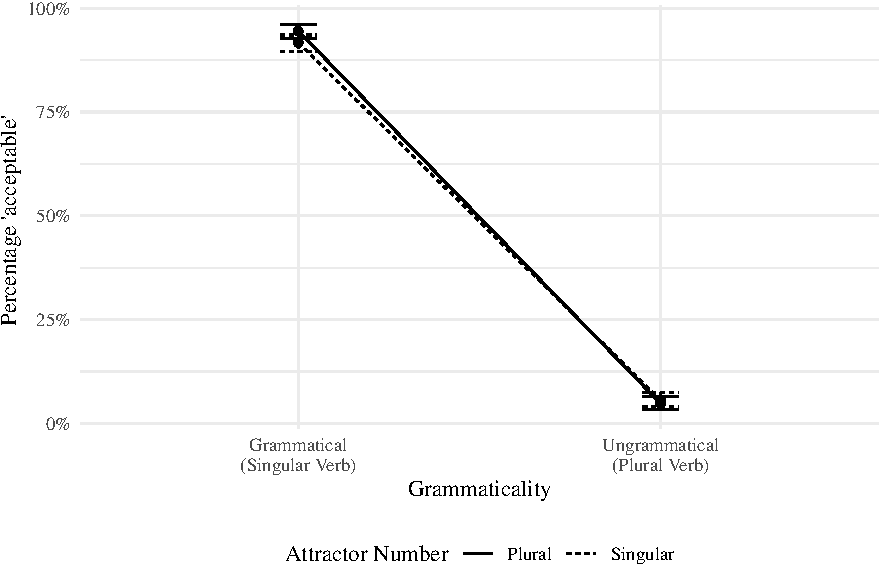
\includegraphics[keepaspectratio]{paper_files/figure-pdf/exp1-condition-means-1.pdf}}

}

\caption{Mean proportion of `acceptable' responses by grammaticality and
attractor number. Error bars show 95\% Clopper--Pearson confidence
intervals.}

\end{figure}%

These descriptive trends were confirmed by our Bayesian mixed-effects
models implemented in brms, assuming a Bernoulli logit link. The model
was fitted to the binary \emph{yes/no} responses and included fixed
effects for Grammaticality and Attractor Number and their interaction,
and random intercepts and slopes for both subjects and items.

Posterior estimates are summarized in Figure 2. The model revealed a
positive effect of grammaticality (\(\beta\) = 5.92 {[}5.41, 6.46{]},
P(\(\beta\) \textgreater{} 1.00)), but no reliable main effect of
attractor number (\(\beta\) = 0.15 {[}-0.19, 0.51{]}, P(\(\beta\)
\textgreater{} 0.81)). On the other hand, there was a small but positive
interaction (\(\beta\) = 0.66 {[}-0.02, 1.38{]}, P(\(\beta\)
\textgreater{} 0.97)). To clarify the effects' presence in grammaticals
only, we fitted two more models that is fitted to the subset of the
data. While the model fitted to grammatical conditions only showed an
effect of attractor number (\(\beta\) = 0.51 {[}0.06, 1.00{]},
P(\(\beta\) \textgreater{} 0.99)), the model fitted to ungrammatical
conditions did not provide evidence for the effect of number
manipulation (\(\beta\) = -0.05 {[}-0.45, 0.37{]}, P(\(\beta\)
\textgreater{} 0.99)). These results suggest that the presence of a
plural attractor did not increase the acceptability of ungrammatical
sentences, nor was this relationship modulated by grammaticality.

\begin{figure}[H]

{\centering \pandocbounded{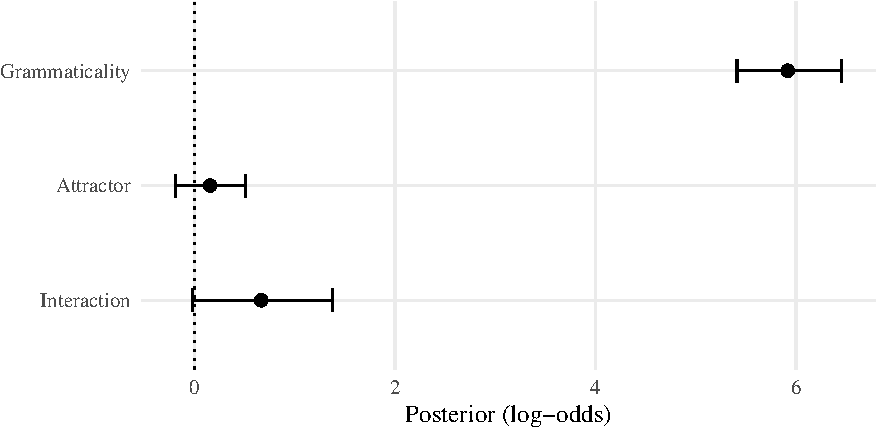
\includegraphics[keepaspectratio]{paper_files/figure-pdf/exp1-fixed-effects-1.pdf}}

}

\caption{Posterior means and 95\% credible intervals for fixed effects
in the two Bayesian models. The x-axis shows the posterior mean
(log-odds scale). The blue intervals correspond to the model in which a
positive interaction was assumed, and the orange intervals to the model
in which it was not.}

\end{figure}%

\subsection{Discussion}\label{discussion}

Experiment 1 tested whether phonological overlap between nominal and
verbal plural morphemes in Turkish induces agreement attraction. The
results provided no evidence for attraction driven by surface-form
similarity. Ungrammatical sentences with plural-marked verbs were not
judged more acceptable when the relative clause verb contained a plural
morpheme. Instead, participants reliably rejected such sentences
regardless of attractor number. This indicates that the verbal plural
marker -lAr does not create the same type of interference observed with
nominal plural attractors in previous studies.

Unexpectedly, grammatical sentences with singular attractors were judged
less acceptable than those with plural attractors. This effect is
unlikely to reflect agreement attraction, since it arises in the
opposite direction. One possibility is that it results from an
interaction between plausibility and referential availability. The
plural morpheme can license a more general interpretation by allowing an
arbitrary or unspecific reference, whereas the singular reduced relative
clause more strongly invites a specific referent, which may be less
accessible in the context of the task. In other words, plural morphology
may facilitate an \emph{arbitrary PRO} interpretation of the embedded
clause, in which the understood subject of the relative clause is not
controlled by any overt antecedent and has a generic or impersonal
reference. A similar effect can be seen in English sentences like `Just
to sit there should be forbidden.' Here, the subject of the infinitival
clause has arbitrary reference. We do not pursue this explanation
further, as it falls outside the scope of the present paper.

One possible reason for the absence of attraction may lie in the
within-experiment statistics. Previous work has shown that participants'
global expectations about the frequency of grammatical and ungrammatical
sentences can alter attraction patterns. \citet{HammerlyEtAl2019} and
\citet{Turk2022} demonstrated that reducing the proportion of
grammatical trials led to attraction effects even in otherwise
grammatical sentences. Similarly, \citet{ArehalliWittenberg2021}
reported that filler distribution affects error correction rates. It is
possible that the current experiment's distribution discouraged
attraction: if participants rarely encountered conditions that supported
attraction, they may have maintained a strong bias against plural-marked
verbs, reinforcing this bias throughout the session.

To test this possibility, Experiment 2 introduced additional conditions
that have previously been shown to elicit attraction in Turkish
\citep{TurkLogacev2024, LagoEtAl2019}. This allowed us to assess whether
the inclusion of genuine nominal attractors modulates the likelihood of
errors and whether participants adapt to the statistical environment of
the task.

\section{Experiment 2: Testing Within-Experiment Statistical
Sensitivity}\label{experiment-2-testing-within-experiment-statistical-sensitivity}

\subsection{Participants}\label{participants-1}

We recruited 95 undergraduate students to participate in the experiment
in exchange for course credit. All participants were native Turkish
speakers, with an average age of 21 (range: 18 -- 30). The experiment
was carried out following the principles of the Declaration of Helsinki
and the regulations concerning research ethics at Bogazici University.
All participants provided informed consent before their participation
and their identities were completely anonymised.

\subsection{Materials}\label{materials-1}

The same materials were used with Exp1. We added items from
\citet{TurkLogacev2024} as an additional condition for nominal cases.

\subsection{Procedures}\label{procedures-1}

The same procedure with Experiment 1 was used.

\subsection{Analysis and Results}\label{analysis-and-results-1}

Participants showed high accuracy in both grammatical (M = 0.95, CI =
{[}0.94,0.96{]}) and ungrammatical filler sentences (M = 0.94, CI =
{[}0.93,0.95{]}), indicating that they understood the task and performed
it reliably.

Figure 3 presents the overall means and credible intervals for `yes'
responses across experimental conditions, as well as the previous data
from \citet{TurkLogacev2024}, which is quite similar to the magnitude of
\citet{LagoEtAl2019}. As shown, in our study, participant gave more
`yes' responses to ungrammatical sentences with plural genitive-marked
nominal attractors (M = 0.12, CI = {[}0.09,0.15{]}) compared to their
singular counterparts (M = 0.12, CI = {[}0.09,0.15{]}).

However, similar increase in acceptability was not found with relative
clause attractors (M = 0.05 and 0.05, CI = {[}0.03, 0.07{]} and {[}0.03,
0.07{]} for singular and plural attractors, respectively). Participants
rated grammatical sentences similarly independent of the attractor
number or attractor type.

\begin{figure}[H]

{\centering \pandocbounded{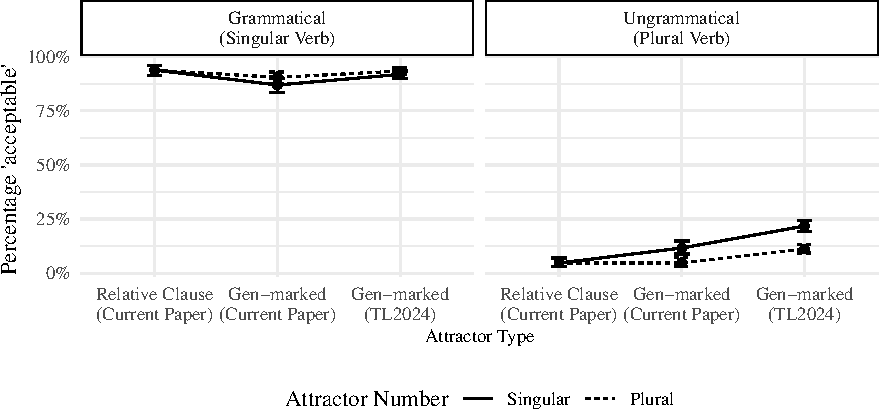
\includegraphics[keepaspectratio]{paper_files/figure-pdf/exp2-condition-means-1.pdf}}

}

\caption{Mean proportion of `acceptable' responses by grammaticality,
attractor number and attractor type. Error bars show 95\%
Clopper--Pearson confidence intervals.}

\end{figure}%

Our models also showed similar results, assuming a Bernoulli logit link.
Our main research question was whether verbal attractors induced
attraction effects. We also wanted to check whether within-experiment
statistics affected the attraction magnitudes, i.e.~the effect of
presence of verbal attractors on nominal attractors. To that end, we
included genitive marked nominals from data from our experiment and
\citet{TurkLogacev2024}. The model was fitted to the binary
\emph{yes/no} responses and included fixed effects for Grammaticality,
Attractor Number, and Attractor Type and their interaction, along with
random intercepts and slopes for both subjects and items.

We present posterior summaries of estimated regression effects from our
model in Figure 4. We found a robust attraction in both nominal
attractor cases, with strongly negative effects for our nominal items (M
= -1.45, CI = {[}-2.12, -0.78{]}, P(\textless0) = \textgreater0.99) and
items from \citet{TurkLogacev2024} (M = -1.16, CI = {[}-1.63, -0.68{]},
P(\textless0) = \textgreater0.99). More importantly, our model found no
evidence for an attraction in verbal attractor conditions (M = 0.08, CI
= {[}-0.7, 0.86{]}, P(\textless0) = 0.44), verifying our observations in
the descriptive statistics. The evidence for a difference in magnitude
of attraction between the two genitive types was not found (M = -0.29,
CI = {[}-1.08, 0.51{]}, P(\textless0) = 0.72), suggesting the
within-experimental distribution did not affect attraction magnitudes.
Finally, we found strong evidence for a decreased overall acceptability
for nominal items in our experiment (M = -1.1, CI = {[}-1.79, -0.44{]},
P(\textless0) = \textgreater0.99), suggesting the within-experimental
distribution did affect overall acceptability, but not attraction.

\begin{figure}[H]

{\centering \pandocbounded{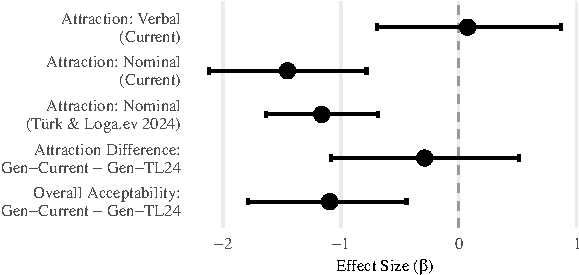
\includegraphics[keepaspectratio]{paper_files/figure-pdf/exp2-fixed-effects-1.pdf}}

}

\caption{Posterior summaries of attraction-related effects. Points
indicate posterior means, and horizontal bars show 95\% credible
intervals on the log-odds (β) scale. Attraction was estimated as the
interaction between grammaticality and attractor number within each
attractor type. Negative values indicate stronger attraction (a reduced
ungrammaticality penalty in plural-attractor conditions). Dashed line
denotes zero (no effect).}

\end{figure}%

\subsection{Discussion}\label{discussion-1}

Experiment 2 tested whether the reason we did not find attraction
effects in Experiment 1 was due to the lack of attraction-inducing
conditions. Our results showed that attraction effects in verbal
attractor condition, purely phonological overlap, did not surface even
when there are robust attraction-inducing trials. Participants reliably
rejected ungrammatical sentences with verbal attractors regardless of
attractor number.

Our results and between experiment comparison showed that
within-experiment statistics, i.e.~exposure to verbal attraction
conditions attraction items, did not substantially reduced the magnitude
of the attraction effects. However, the overall acceptability in our
nominal attractor elements were reduced compared to the trials from
\citet{TurkLogacev2024}. This is inline with previous findings that
shows participants' judgments within the experiment are modulated by the
distribution of trials. Interestingly, previous studies achieved this
with instructions or filler elements
\citep{HammerlyEtAl2019, ArehalliWittenberg2021}. We show that the
experimental conditions and the presence of an effect within a subset of
conditions also plays a role in modulating overall acceptability.

\section{General Discussion}\label{general-discussion}

In two high-powered speeded acceptability judgment experiments, we
tested whether pure phonological overlap between agreement morphemes can
elicit agreement attraction. Our goal was to evaluate previous accounts
that attribute attraction to accidental or non-accidental syncretism
between forms that can serve as agreement controllers. Turkish provides
a useful test case because the plural suffix -lAr appears both on verbs
and on nouns, but only nominal -lAr can control agreement. If
phonological overlap alone can activate controller-relevant cues, then
plural-marked verbs embedded in reduced relative clauses should induce
attraction effects even though they cannot syntactically control
agreement.

Across both experiments, we found that Turkish attraction is determined
by being a potential controller rather than merely resembling one.
Participants did not produce or endorse attraction errors in sentences
containing verbal attractors, and this absence of attraction persisted
even when the same participants showed robust attraction with nominal
attractors in the same session.

These results indicate that attraction depends on abstract feature
overlap with potential controllers, not on surface-form similarity. This
pattern converges with prior results in English and Turkish that failed
to find attraction for pseudoplural or phonologically plural forms
\citep{BockEberhard1993, HaskellMacDonald2003, NicolEtAl:2016}, and
stands in contrast to findings from Russian \citep{Slioussar2018}.

In \citet{Slioussar2018}, genitive-marked singular nouns that were
homophonous with nominative plurals elicited greater attraction effects
than their genitive-plural counterparts. This is striking because the
relevant nouns lacked a plural feature that could percolate or serve as
a retrieval cue. The effect was therefore interpreted as evidence that
comprehenders can use phonological form to activate abstract agreement
features. However, it is important to note that the evidence for
phonological attraction in Russian rests on a small empirical base. The
production and comprehension experiments in \citep{Slioussar2018}
included only 32 participants each, and the attraction effects were
derived from a small number of error trials (13 in production and 18 in
comprehension). Given the low number of critical observations, such
effects are vulnerable to sampling variability and may not generalize
beyond that dataset.

The high-powered Turkish results challenge that interpretation. Despite
identical surface overlap between verbal and nominal plural morphology,
phonological similarity alone did not yield attraction. This
cross-linguistic contrast suggests that form-based activation of
agreement features is not a universal property of the parsing system
but, at best, depends on language-specific mappings between morphology
and syntactic function \citep{DillonKeshev2024}.

A more plausible account is that attraction is modulated by the
availability of morphosyntactic features that can signal controllerhood.
Syncretism contributes to attraction only when one of the syncretic
forms can legitimately control agreement or share features with the
target. In other words, it is not form overlap per se, but feature
ambiguity that matters. This interpretation aligns with cross-linguistic
findings showing that attraction is strongest when the attractor bears
case or number morphology that is sometimes associated with subjects or
agreement controllers
\citep{LagoEtAl2019, BhatiaDillon2022, BleotuDillon2024, HartsuikerEtAl2003}.
Earlier formulations of these models left open whether `looking like' a
controller or `being able to be' a controller was critical. The present
results favor the latter: only morphologically licensed controllers
engage in attraction.

\section*{References}\label{references}
\addcontentsline{toc}{section}{References}

\newcommand{\doi}[1]{\href{http://dx.doi.org/#1}{http://dx.doi.org/#1}}
\begingroup
\raggedright
\singlespacing

\renewcommand{\bibsection}{}
\bibliography{bibliography.bib}

\endgroup





\end{document}
